\documentclass[11pt,a4paper]{article}
\usepackage[utf8]{inputenc}
\usepackage[T1]{fontenc}
\usepackage{geometry}
\usepackage{graphicx}
\usepackage{xcolor}
\usepackage{hyperref}
\usepackage{tikz}
\usetikzlibrary{shapes,arrows,positioning,calc,shadows,fit,backgrounds}
\usepackage{enumitem}
\usepackage{fancyhdr}
\usepackage{tcolorbox}
\usepackage{tabularx}
\usepackage{booktabs}
\usepackage{multicol}
\usepackage{listings}
\usepackage{amsmath}
\usepackage{colortbl}

\geometry{margin=0.75in}

% Define colors
\definecolor{primaryblue}{RGB}{33, 150, 243}
\definecolor{accentblue}{RGB}{25, 118, 210}
\definecolor{darkblue}{RGB}{13, 71, 161}
\definecolor{gpu0color}{RGB}{76, 175, 80}
\definecolor{gpu1color}{RGB}{255, 152, 0}
\definecolor{lightgray}{RGB}{245, 245, 245}
\definecolor{codebg}{RGB}{250, 250, 250}

\hypersetup{
    colorlinks=true,
    linkcolor=darkblue,
    filecolor=darkblue,
    urlcolor=primaryblue,
    pdftitle={llamatelemetry v0.1.0 Portfolio - Waqas Muhammad},
    pdfauthor={Waqas Muhammad}
}

\pagestyle{fancy}
\fancyhf{}
\renewcommand{\headrulewidth}{0.4pt}
\fancyhead[L]{\textcolor{primaryblue}{\small llamatelemetry v0.1.0 Portfolio}}
\fancyhead[R]{\textcolor{darkblue}{\small Waqas Muhammad}}
\fancyfoot[C]{\textcolor{gray}{\small Page \thepage}}
\fancyfoot[R]{\textcolor{primaryblue}{\small llamatelemetry.github.io}}

% Code listing style
\lstset{
    basicstyle=\small\ttfamily,
    backgroundcolor=\color{codebg},
    frame=single,
    breaklines=true,
    columns=fullflexible
}

\begin{document}

% ============================================
% TITLE PAGE
% ============================================
\begin{titlepage}
    \centering
    \vspace*{1cm}

    {\Huge\bfseries\textcolor{primaryblue}{llamatelemetry v0.1.0}\par}
    \vspace{0.3cm}
    {\Large CUDA 12 Inference Backend for Unsloth\par}
    \vspace{0.2cm}
    {\large\textit{Split-GPU Architecture on Kaggle Dual Tesla T4}\par}

    \vspace{1.5cm}

    % Project highlight box
    \begin{tcolorbox}[colback=primaryblue!10,colframe=primaryblue,width=0.85\textwidth,arc=3mm,boxrule=1mm]
        \centering
        \large
        \textbf{Flagship Achievement}\\[0.3cm]
        \Large\textbf{\textcolor{accentblue}{GGUF Neural Network Visualization}}\\[0.2cm]
        \normalsize
        8 Interactive Graphistry Dashboards • 929 Nodes • 981 Edges\\
        896 Attention Heads • Dual-GPU Architecture
    \end{tcolorbox}

    \vspace{1.5cm}

    % Key metrics
    \begin{tcolorbox}[colback=white,colframe=accentblue,width=0.9\textwidth,arc=2mm]
        \begin{center}
        \textbf{\Large Project Highlights}
        \vspace{0.4cm}

        \begin{tabular}{ccc}
            \textbf{\LARGE\textcolor{gpu0color}{GPU 0}} &
            \textbf{\LARGE\textcolor{gpu1color}{GPU 1}} &
            \textbf{\LARGE\textcolor{primaryblue}{11 Notebooks}} \\
            LLM Inference & Graphistry Viz & Kaggle Tutorials \\[0.5cm]

            \textbf{\LARGE\textcolor{accentblue}{929}} &
            \textbf{\LARGE\textcolor{accentblue}{981}} &
            \textbf{\LARGE\textcolor{accentblue}{896}} \\
            Graph Nodes & Graph Edges & Attention Heads \\[0.5cm]

            \textbf{\LARGE\textcolor{accentblue}{28}} &
            \textbf{\LARGE\textcolor{accentblue}{1.88 GB}} &
            \textbf{\LARGE\textcolor{accentblue}{5.6×}} \\
            Transformer Layers & Q4\_K\_M Model & Compression \\
        \end{tabular}
        \end{center}
    \end{tcolorbox}

    \vspace{1.5cm}

    % Author info
    \begin{tcolorbox}[colback=lightgray,colframe=gray,width=0.75\textwidth,arc=2mm]
        \centering
        \textbf{Waqas Muhammad}\\
        GPU Systems Engineer | CUDA Specialist\\[0.3cm]
        \href{mailto:waqasm86@gmail.com}{waqasm86@gmail.com}\\
        \href{https://github.com/waqasm86}{github.com/waqasm86}\\
        \href{https://llamatelemetry.github.io}{llamatelemetry.github.io}
    \end{tcolorbox}

    \vfill

    {\small\textcolor{gray}{Portfolio Date: January 2026}}
\end{titlepage}

% ============================================
% TABLE OF CONTENTS
% ============================================
\tableofcontents
\newpage

% ============================================
% SECTION 1: EXECUTIVE SUMMARY
% ============================================
\section{Executive Summary}

\textbf{llamatelemetry v0.1.0} is a production-ready CUDA 12 inference backend specifically engineered for deploying small GGUF models (1B-5B parameters) on \textbf{Kaggle's dual Tesla T4 GPUs} (30GB total VRAM). The project introduces an innovative \textbf{split-GPU architecture} where GPU 0 handles LLM inference via llama.cpp's llama-server, while GPU 1 powers RAPIDS cuGraph and Graphistry for real-time neural network visualization.

\subsection{Core Innovation}

The flagship achievement is \textbf{Notebook 11: GGUF Neural Network Visualization}, which demonstrates groundbreaking capabilities:

\begin{itemize}[leftmargin=*]
    \item \textbf{8 Interactive Graphistry Dashboards} showcasing internal GGUF model architecture
    \item \textbf{929 nodes} representing Llama-3.2-3B components (layers, attention heads, embeddings)
    \item \textbf{981 edges} showing data flow and connections between components
    \item \textbf{896 attention heads} visualized across 28 transformer layers
    \item \textbf{GPU-accelerated PageRank \& Centrality} analysis via RAPIDS cuGraph
    \item \textbf{Split-GPU orchestration} enabling simultaneous inference and visualization
\end{itemize}

\subsection{Business Value \& Impact}

\begin{tcolorbox}[colback=primaryblue!5,colframe=primaryblue,arc=2mm]
\textbf{Key Achievements:}
\begin{itemize}[nosep]
    \item First CUDA 12 backend specifically designed for Unsloth's GGUF export workflow
    \item Novel split-GPU architecture enabling LLM + visualization on free Kaggle infrastructure
    \item 11 comprehensive tutorial notebooks (beginner to advanced) with complete documentation
    \item Production-ready Python SDK with 961MB pre-built CUDA binaries (zero compilation)
    \item Open-source with MIT license, actively maintained at \href{https://github.com/llamatelemetry/llamatelemetry}{github.com/llamatelemetry/llamatelemetry}
\end{itemize}
\end{tcolorbox}

\subsection{Technical Highlights}

\begin{multicols}{2}
\textbf{Platform \& Hardware}
\begin{itemize}[nosep]
    \item Kaggle dual Tesla T4 (15GB × 2)
    \item CUDA 12.x with SM 7.5 support
    \item FlashAttention optimization
    \item Tensor Core utilization
\end{itemize}

\textbf{Model Support}
\begin{itemize}[nosep]
    \item 1B-5B parameter range
    \item 29 GGUF quantization formats
    \item Q4\_K\_M, Q5\_K\_M, IQ3\_XS
    \item Llama, Gemma, Qwen, Mistral
\end{itemize}

\textbf{Integration Ecosystem}
\begin{itemize}[nosep]
    \item Unsloth fine-tuning workflow
    \item llama.cpp server (build 7760)
    \item RAPIDS cuDF \& cuGraph 25.6
    \item Graphistry cloud visualization
\end{itemize}

\textbf{Developer Experience}
\begin{itemize}[nosep]
    \item Python 3.11+ SDK
    \item OpenAI-compatible API
    \item MkDocs documentation site
    \item Comprehensive error handling
\end{itemize}
\end{multicols}

\newpage

% ============================================
% SECTION 2: PROJECT ARCHITECTURE
% ============================================
\section{Project Architecture}

\subsection{Split-GPU Design Philosophy}

llamatelemetry v0.1.0 introduces a novel \textbf{split-GPU architecture pattern} optimized for Kaggle's dual T4 environment. This design enables simultaneous LLM inference and GPU-accelerated visualization without resource contention.

\begin{figure}[h]
\centering
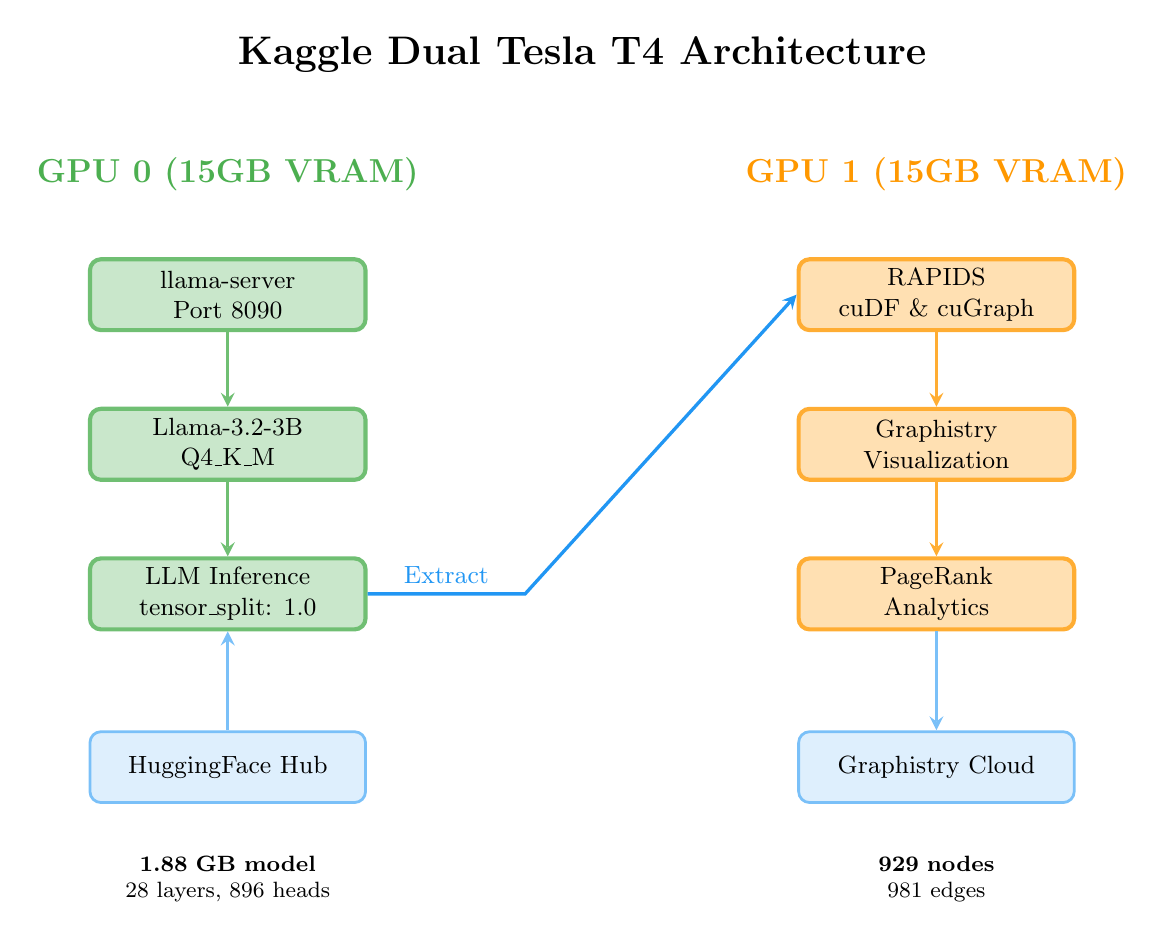
\begin{tikzpicture}[
    node distance=2cm,
    box/.style={rectangle, draw, thick, rounded corners, minimum width=3.5cm, minimum height=0.9cm, align=center, font=\small},
    gpu0/.style={box, fill=gpu0color!30, draw=gpu0color!80, line width=1.5pt},
    gpu1/.style={box, fill=gpu1color!30, draw=gpu1color!80, line width=1.5pt},
    external/.style={box, fill=primaryblue!15, draw=primaryblue!60, line width=1pt, minimum width=3.5cm},
    arrow/.style={->, >=stealth, thick, line width=1.2pt}
]

% Title
\node[above, font=\Large\bfseries] at (0,9) {Kaggle Dual Tesla T4 Architecture};

% GPU 0 Column (Left) - x=-4.5 for wider spacing
\node[above, font=\large\bfseries, gpu0color] at (-4.5,7.5) {GPU 0 (15GB VRAM)};
\node[gpu0] (llama) at (-4.5,6.3) {llama-server\\Port 8090};
\node[gpu0] (model) at (-4.5,4.4) {Llama-3.2-3B\\Q4\_K\_M};
\node[gpu0] (inference) at (-4.5,2.5) {LLM Inference\\tensor\_split: 1.0};

% GPU 1 Column (Right) - x=4.5 for wider spacing
\node[above, font=\large\bfseries, gpu1color] at (4.5,7.5) {GPU 1 (15GB VRAM)};
\node[gpu1] (rapids) at (4.5,6.3) {RAPIDS\\cuDF \& cuGraph};
\node[gpu1] (graphistry) at (4.5,4.4) {Graphistry\\Visualization};
\node[gpu1] (analytics) at (4.5,2.5) {PageRank\\Analytics};

% Vertical arrows within columns - use .south and .north for precise connections
\draw[arrow, gpu0color!80] (llama.south) -- (model.north);
\draw[arrow, gpu0color!80] (model.south) -- (inference.north);
\draw[arrow, gpu1color!80] (rapids.south) -- (graphistry.north);
\draw[arrow, gpu1color!80] (graphistry.south) -- (analytics.north);

% External connections - positioned lower
\node[external] (hf) at (-4.5,0.3) {HuggingFace Hub};
\node[external] (cloud) at (4.5,0.3) {Graphistry Cloud};

% HuggingFace Hub arrow - UPWARD (bottom to top direction)
\draw[arrow, primaryblue!60] (hf.north) -- (inference.south);

% Cross-GPU data flow - pure horizontal path
\draw[arrow, primaryblue] (inference.east) -- ++(2,0) node[above, pos=0.5, font=\small] {Extract} -- (rapids.west);

% Graphistry Cloud arrow - DOWNWARD (top to bottom direction) - FIXED DIRECTION
\draw[arrow, primaryblue!60] (analytics.south) -- (cloud.north);

% Bottom labels
\node[below, text width=3.5cm, align=center, font=\footnotesize] at (-4.5,-0.7) {\textbf{1.88 GB model}\\28 layers, 896 heads};
\node[below, text width=3.5cm, align=center, font=\footnotesize] at (4.5,-0.7) {\textbf{929 nodes}\\981 edges};

\end{tikzpicture}
\caption{llamatelemetry v0.1.0 Split-GPU Architecture on Kaggle Dual T4}
\end{figure}

\newpage

% ============================================
% SECTION 3: TUTORIAL NOTEBOOKS OVERVIEW
% ============================================
\section{Tutorial Notebooks (01-10): Core Capabilities}

llamatelemetry v0.1.0 includes 11 comprehensive Kaggle notebooks that progressively build expertise from beginner to advanced topics. Notebooks 01-10 establish foundational skills, while Notebook 11 (detailed in Section 4) demonstrates the flagship visualization capabilities.

\subsection{Learning Path Structure}

\begin{figure}[h]
\centering
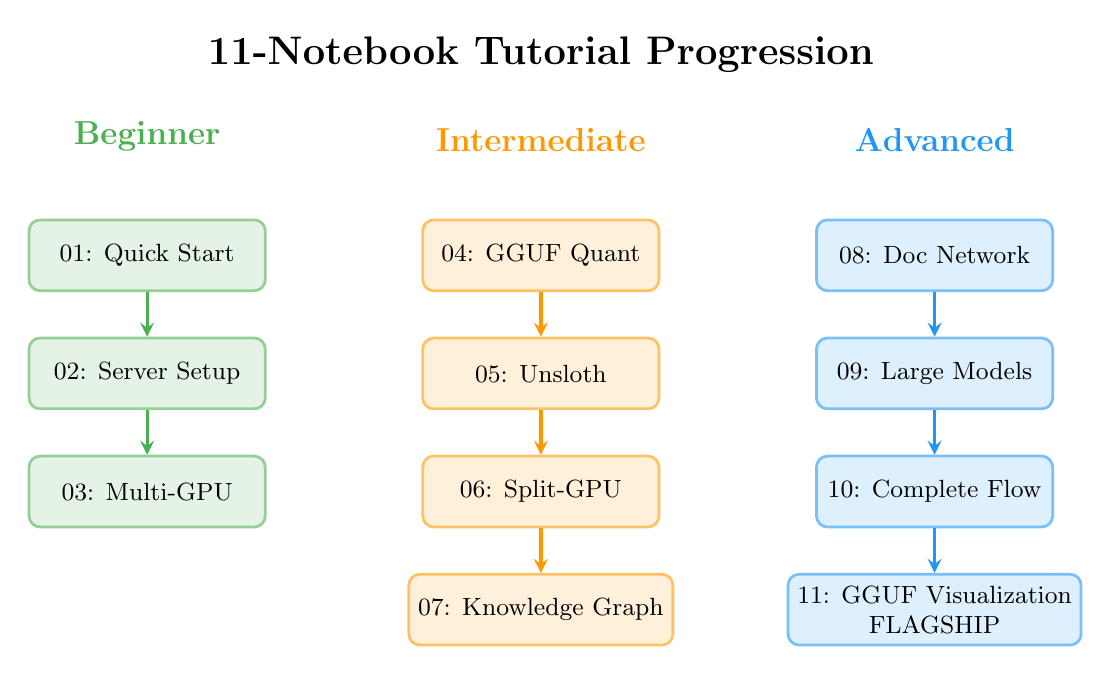
\begin{tikzpicture}[
    node distance=1.5cm and 2.5cm,
    level/.style={rectangle, draw, thick, rounded corners, minimum width=3cm, minimum height=0.9cm, align=center, fill=white, font=\small},
    beginner/.style={level, fill=gpu0color!15, draw=gpu0color!60, line width=1pt},
    intermediate/.style={level, fill=gpu1color!15, draw=gpu1color!60, line width=1pt},
    advanced/.style={level, fill=primaryblue!15, draw=primaryblue!60, line width=1pt},
    arrow/.style={->, >=stealth, thick, line width=1.2pt}
]

% Title
\node[above, font=\Large\bfseries] at (0,7) {11-Notebook Tutorial Progression};

% Beginner Level - Left Column
\node[above, font=\large\bfseries, gpu0color] at (-5,6) {Beginner};
\node[beginner] (nb01) at (-5,4.8) {01: Quick Start};
\node[beginner] (nb02) at (-5,3.3) {02: Server Setup};
\node[beginner] (nb03) at (-5,1.8) {03: Multi-GPU};

% Intermediate Level - Middle Column
\node[above, font=\large\bfseries, gpu1color] at (0,6) {Intermediate};
\node[intermediate] (nb04) at (0,4.8) {04: GGUF Quant};
\node[intermediate] (nb05) at (0,3.3) {05: Unsloth};
\node[intermediate] (nb06) at (0,1.8) {06: Split-GPU};
\node[intermediate] (nb07) at (0,0.3) {07: Knowledge Graph};

% Advanced Level - Right Column
\node[above, font=\large\bfseries, primaryblue] at (5,6) {Advanced};
\node[advanced] (nb08) at (5,4.8) {08: Doc Network};
\node[advanced] (nb09) at (5,3.3) {09: Large Models};
\node[advanced] (nb10) at (5,1.8) {10: Complete Flow};
\node[advanced] (nb11) at (5,0.3) {11: GGUF Visualization\\FLAGSHIP};

% Vertical arrows within columns (direct connections)
\draw[arrow, gpu0color] (nb01.south) -- (nb02.north);
\draw[arrow, gpu0color] (nb02.south) -- (nb03.north);
\draw[arrow, gpu1color] (nb04.south) -- (nb05.north);
\draw[arrow, gpu1color] (nb05.south) -- (nb06.north);
\draw[arrow, gpu1color] (nb06.south) -- (nb07.north);
\draw[arrow, primaryblue] (nb08.south) -- (nb09.north);
\draw[arrow, primaryblue] (nb09.south) -- (nb10.north);
\draw[arrow, primaryblue] (nb10.south) -- (nb11.north);

\end{tikzpicture}
\caption{Progressive Learning Path Through 11 Tutorial Notebooks}
\end{figure}

\subsection{Notebooks 01-10: Detailed Breakdown}

\begin{table}[h]
\centering
\small
\begin{tabularx}{\textwidth}{|c|l|X|r|}
\hline
\rowcolor{primaryblue!20}
\textbf{\#} & \textbf{Notebook} & \textbf{Key Skills Demonstrated} & \textbf{Time} \\
\hline
\multicolumn{4}{|c|}{\cellcolor{gpu0color!20}\textbf{Beginner: Foundation}} \\
\hline
01 & Quick Start & Basic llamatelemetry setup, model loading, simple inference & 5 min \\
\hline
02 & Server Setup & llama-server lifecycle, configuration, API usage & 15 min \\
\hline
03 & Multi-GPU & Dual T4 detection, tensor\_split, layer distribution & 20 min \\
\hline
\multicolumn{4}{|c|}{\cellcolor{gpu1color!20}\textbf{Intermediate: Integration}} \\
\hline
04 & GGUF Quantization & K-quants vs I-quants, VRAM estimation, format selection & 20 min \\
\hline
05 & Unsloth Integration & Fine-tune → GGUF export → llamatelemetry deployment & 30 min \\
\hline
06 & Split-GPU Graphistry & GPU 0 (LLM) + GPU 1 (Graphistry) orchestration & 30 min \\
\hline
07 & Knowledge Graphs & Entity extraction, relationship detection, graph viz & 30 min \\
\hline
\multicolumn{4}{|c|}{\cellcolor{primaryblue!20}\textbf{Advanced: Production}} \\
\hline
08 & Document Networks & Similarity analysis, community detection, cuGraph & 35 min \\
\hline
09 & Large Models & 13B+ model deployment, memory optimization & 30 min \\
\hline
10 & Complete Workflow & End-to-end pipeline: setup → inference → viz → API & 50 min \\
\hline
\end{tabularx}
\caption{Notebooks 01-10: Comprehensive Skill Development Path}
\end{table}

\subsection{Technical Skills Progression}

By completing notebooks 01-10, users master:

\begin{multicols}{2}
\textbf{GPU Management}
\begin{itemize}[nosep]
    \item Dual T4 detection
    \item CUDA\_VISIBLE\_DEVICES
    \item Memory profiling
    \item Performance monitoring
\end{itemize}

\textbf{LLM Deployment}
\begin{itemize}[nosep]
    \item GGUF model loading
    \item llama-server config
    \item API client usage
    \item Batch inference
\end{itemize}

\textbf{Multi-GPU Techniques}
\begin{itemize}[nosep]
    \item Tensor-split ratios
    \item Layer distribution
    \item FlashAttention
    \item NCCL vs tensor-split
\end{itemize}

\textbf{Visualization Stack}
\begin{itemize}[nosep]
    \item RAPIDS cuGraph
    \item Graphistry dashboards
    \item Knowledge graph construction
    \item GPU-accelerated analytics
\end{itemize}
\end{multicols}

These notebooks prepare users for the advanced capabilities demonstrated in Notebook 11, which synthesizes all learned techniques into a production-grade neural network visualization system.

\newpage

% ============================================
% SECTION 4: NOTEBOOK 11 - FLAGSHIP ACHIEVEMENT
% ============================================
\section{Notebook 11: GGUF Neural Network Visualization}

\begin{tcolorbox}[colback=accentblue!10,colframe=accentblue,title={\Large\textbf{FLAGSHIP ACHIEVEMENT: GGUF Neural Network Visualization}},arc=3mm,boxrule=1.5mm]
\large
\textbf{File:} \texttt{11-gguf-neural-network-graphistry-vis-executed-2.ipynb}

\vspace{0.3cm}
\normalsize
The culminating demonstration of llamatelemetry v0.1.0's capabilities, showcasing a groundbreaking approach to visualizing the internal architecture of GGUF quantized models through 8 interactive Graphistry dashboards.

\vspace{0.3cm}
\textbf{Key Achievement:} First tool to visualize GGUF quantization as interactive graphs with GPU-accelerated PageRank analysis, revealing the internal structure of transformer models in unprecedented detail.
\end{tcolorbox}

\subsection{Executive Overview}

Notebook 11 demonstrates \textbf{advanced neural network architecture visualization} by extracting the complete structural graph of Llama-3.2-3B-Instruct (Q4\_K\_M quantization) and rendering it through 8 distinct interactive dashboards hosted on Graphistry cloud.

\textbf{Business Value:}
\begin{itemize}[leftmargin=*]
    \item \textbf{AI Explainability}: Makes "black box" transformer models transparent and explorable
    \item \textbf{Model Validation}: Verify GGUF conversions match original HuggingFace architectures
    \item \textbf{Research Applications}: Identify pruning opportunities, analyze information flow, compare quantization strategies
    \item \textbf{Educational Tool}: Visual understanding of transformer attention mechanisms and layer interactions
\end{itemize}

\textbf{Technical Innovation:}
\begin{itemize}[leftmargin=*]
    \item Runtime introspection (no binary parsing) - architecture extracted via API queries
    \item Dual-GPU split enables simultaneous inference and visualization
    \item Graph theory metrics (PageRank) applied to neural network components
    \item Zero-code dashboard generation from pandas DataFrames
\end{itemize}

\subsection{Model Architecture: Llama-3.2-3B-Instruct}

\begin{table}[h]
\centering
\begin{tabularx}{\textwidth}{|l|X|}
\hline
\rowcolor{primaryblue!20}
\textbf{Specification} & \textbf{Value} \\
\hline
\textbf{Model} & Llama-3.2-3B-Instruct (bartowski/Llama-3.2-3B-Instruct-GGUF) \\
\hline
\textbf{Quantization} & Q4\_K\_M (4-bit k-quants, medium variant) \\
\hline
\textbf{Original Size} & $\sim$10.6 GB (FP32) \\
\hline
\textbf{Quantized Size} & \textbf{1.88 GB} \\
\hline
\textbf{Compression Ratio} & \textbf{5.6×} \\
\hline
\textbf{Bits Per Parameter} & 5.7 average \\
\hline
\hline
\textbf{Total Parameters} & $\sim$2.8 billion \\
\hline
\textbf{Transformer Layers} & \textbf{28 layers} \\
\hline
\textbf{Attention Heads per Layer} & 32 heads \\
\hline
\textbf{Total Attention Heads} & \textbf{896 heads} (32 × 28) \\
\hline
\textbf{Hidden Dimension} & 3,072 \\
\hline
\textbf{Vocabulary Size} & 128,256 tokens \\
\hline
\textbf{Context Length} & 8,192 tokens (max) \\
\hline
\textbf{FFN Multiplier} & 4× (SwiGLU activation) \\
\hline
\hline
\multicolumn{2}{|c|}{\cellcolor{gpu0color!20}\textbf{Parameter Distribution}} \\
\hline
Embedding Layer & 394M params (12.6\%) \\
\hline
Attention Layers & 1.05B params (33.7\%) \\
\hline
Feed-Forward Layers & 2.1B params (67.2\%) \\
\hline
Output Layer & 394M params (12.6\%) \\
\hline
\end{tabularx}
\caption{Llama-3.2-3B-Instruct Model Specifications}
\end{table}

\newpage

\subsection{Dual-GPU Architecture: Workflow Visualization}

\begin{figure}[h]
\centering
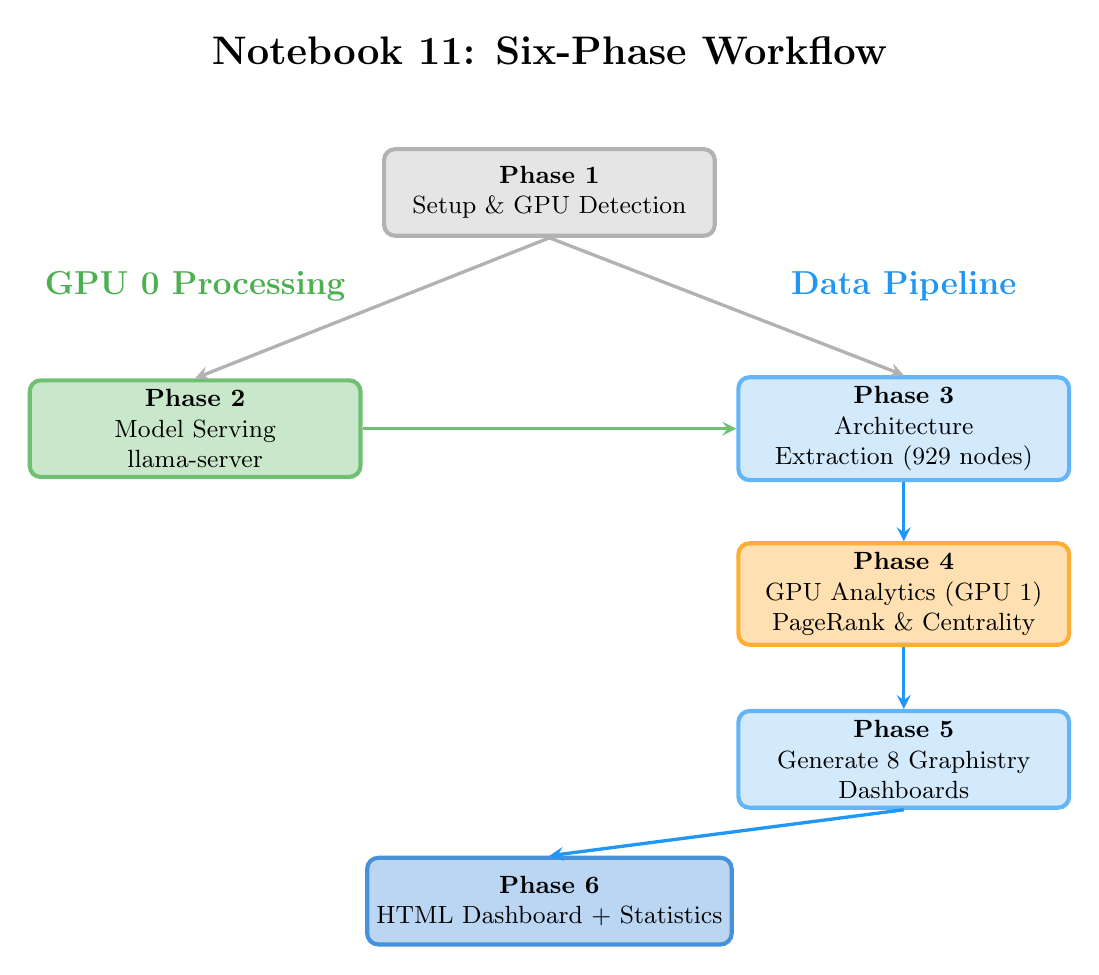
\begin{tikzpicture}[
    node distance=2cm,
    box/.style={rectangle, draw, thick, rounded corners, minimum width=4.2cm, minimum height=1.1cm, align=center, font=\small},
    setup/.style={box, fill=gray!20, draw=gray!60, line width=1.5pt},
    gpu0/.style={box, fill=gpu0color!30, draw=gpu0color!80, line width=1.5pt},
    gpu1/.style={box, fill=gpu1color!30, draw=gpu1color!80, line width=1.5pt},
    process/.style={box, fill=primaryblue!20, draw=primaryblue!70, line width=1.5pt},
    output/.style={box, fill=accentblue!30, draw=accentblue!80, line width=1.5pt},
    arrow/.style={->, >=stealth, thick, line width=1.2pt}
]

% Title
\node[above, font=\Large\bfseries] at (0,9) {Notebook 11: Six-Phase Workflow};

% Phase 1: Setup (centered at top)
\node[setup] (phase1) at (0,7.5) {\textbf{Phase 1}\\Setup \& GPU Detection};

% Left column: GPU 0 Processing
\node[above, font=\large\bfseries, gpu0color] at (-4.5,6) {GPU 0 Processing};
\node[gpu0] (phase2) at (-4.5,4.5) {\textbf{Phase 2}\\Model Serving\\llama-server};

% Right column: Data Pipeline
\node[above, font=\large\bfseries, primaryblue] at (4.5,6) {Data Pipeline};
\node[process] (phase3) at (4.5,4.5) {\textbf{Phase 3}\\Architecture\\Extraction (929 nodes)};
\node[gpu1] (phase4) at (4.5,2.4) {\textbf{Phase 4}\\GPU Analytics (GPU 1)\\PageRank \& Centrality};
\node[process] (phase5) at (4.5,0.3) {\textbf{Phase 5}\\Generate 8 Graphistry\\Dashboards};

% Phase 6: Output (centered at bottom)
\node[output] (phase6) at (0,-1.5) {\textbf{Phase 6}\\HTML Dashboard + Statistics};

% Arrows from Phase 1 - simple straight lines
\draw[arrow, gray!60] (phase1.south) -- (phase2.north);
\draw[arrow, gray!60] (phase1.south) -- (phase3.north);

% Vertical arrows within right column - direct connections
\draw[arrow, primaryblue] (phase3.south) -- (phase4.north);
\draw[arrow, primaryblue] (phase4.south) -- (phase5.north);

% Cross-column data flow - simple straight horizontal line
\draw[arrow, gpu0color!80] (phase2.east) -- (phase3.west);

% Convergence to Phase 6 - simple straight line
\draw[arrow, primaryblue] (phase5.south) -- (phase6.north);

\end{tikzpicture}
\caption{Notebook 11: Complete Workflow from Model Loading to Visualization}
\end{figure}

\subsection{GPU Workload Distribution}

\begin{table}[h]
\centering
\begin{tabularx}{\textwidth}{|l|X|r|}
\hline
\rowcolor{gpu0color!30}
\multicolumn{3}{|c|}{\textbf{GPU 0: Tesla T4 (15GB) - LLM Inference}} \\
\hline
\textbf{Process} & llama-server (Port 8090) & \\
\textbf{Model} & Llama-3.2-3B-Instruct Q4\_K\_M & 1.88 GB \\
\textbf{Config} & tensor\_split="1.0,0.0" (100\% GPU 0) & \\
\textbf{Layers} & 28 transformer layers loaded & \\
\textbf{Context} & 4096 tokens & \\
\textbf{API} & OpenAI-compatible REST endpoint & \\
\textbf{VRAM Used} & 3-4 GB (model + KV cache) & \\
\hline
\hline
\rowcolor{gpu1color!30}
\multicolumn{3}{|c|}{\textbf{GPU 1: Tesla T4 (15GB) - Graph Analytics \& Visualization}} \\
\hline
\textbf{Framework} & RAPIDS cuGraph 25.6 + Graphistry 0.50.4 & \\
\textbf{Data} & 929 nodes, 981 edges & \\
\textbf{Analytics} & PageRank, Betweenness Centrality & \\
\textbf{Rendering} & Graphistry cloud upload & \\
\textbf{VRAM Used} & 0.5-1 GB (graph data + computation) & \\
\hline
\end{tabularx}
\caption{Dual-GPU Workload Isolation in Notebook 11}
\end{table}

\textbf{Why Split-GPU?} This architecture demonstrates \textbf{workload isolation} - keeping expensive model inference separate from compute-intensive graph operations prevents memory contention and GPU thrashing, enabling smooth concurrent operation.

\newpage

\subsection{8 Interactive Graphistry Visualizations}

\begin{tcolorbox}[colback=white,colframe=primaryblue,arc=2mm,title={\textbf{Complete Visualization Suite}}]

\textbf{1. Main Architecture Visualization}\\
\textit{929 nodes, 981 edges}
\begin{itemize}[nosep]
    \item Complete Llama-3.2-3B structure
    \item Color-coded by component type (7 categories: embedding, transformer, attention, FFN, LayerNorm, output)
    \item Node size scaled by PageRank importance
    \item Custom tooltips: parameters, dimensions, centrality metrics
    \item Force-directed layout with configurable gravity
\end{itemize}

\vspace{0.3cm}

\textbf{2-6. Layer-by-Layer Subgraphs (Layers 1-5)}\\
\textit{35 nodes, 34 edges each}
\begin{itemize}[nosep]
    \item Deep-dive into individual transformer blocks
    \item Components: 1 transformer block + 32 attention heads + 2 shared (LayerNorm, FFN)
    \item Interactive filtering by layer number
    \item Detailed parameter counts per attention head
    \item Connection patterns between heads and blocks
\end{itemize}

\vspace{0.3cm}

\textbf{7. Interactive Layer Explorer}\\
\textit{Full 929-node graph with UI controls}
\begin{itemize}[nosep]
    \item Sidebar filtering UI: \texttt{showFilters=true}
    \item Dynamic layer switching: Select any of 28 layers
    \item Label display: \texttt{showLabels=true}
    \item Full sidebar mode for advanced exploration
    \item Export capabilities for further analysis
\end{itemize}

\vspace{0.3cm}

\textbf{8. Quantization Blocks Visualization}\\
\textit{112 nodes (4 blocks × 28 layers)}
\begin{itemize}[nosep]
    \item Q4\_K\_M memory distribution across layers
    \item Each block: $\sim$737K parameters, $\sim$1.2 MB
    \item Visualizes 5.6× compression effect
    \item Shows how quantization reduces memory footprint
    \item Weight distribution analysis
\end{itemize}

\end{tcolorbox}

\subsection{Graph Structure: Component Breakdown}

\begin{table}[h]
\centering
\begin{tabularx}{\textwidth}{|l|r|r|X|}
\hline
\rowcolor{primaryblue!20}
\textbf{Component Type} & \textbf{Count} & \textbf{Edges} & \textbf{Description} \\
\hline
Embedding Layer & 1 & - & Input token embedding (128K vocab) \\
\hline
Transformer Blocks & 28 & 28 & Main transformer layers (Layer 0-27) \\
\hline
Attention Heads & 896 & 896 & 32 heads × 28 layers \\
\hline
LayerNorm & 2 & 28 & Pre/post normalization (shared) \\
\hline
Feed-Forward (FFN) & 1 & 28 & SwiGLU activation (shared) \\
\hline
Output Layer & 1 & 1 & Final prediction head \\
\hline
\hline
\textbf{Total} & \textbf{929} & \textbf{981} & Complete architecture graph \\
\hline
\end{tabularx}
\caption{929-Node Graph: Component Breakdown}
\end{table}

\newpage

\subsection{GPU-Accelerated Analytics: PageRank \& Centrality}

Notebook 11 applies \textbf{graph theory metrics} to the neural network architecture using RAPIDS cuGraph (GPU-accelerated algorithms):

\begin{tcolorbox}[colback=lightgray,colframe=darkblue]
\textbf{PageRank Analysis}\\
Identifies the most "important" components in the network based on connection strength and centrality.

\vspace{0.2cm}
\textbf{Key Findings:}
\begin{itemize}[nosep]
    \item \textbf{Highest PageRank:} Middle-layer attention heads (Layers 12-16)
    \item \textbf{Bottleneck Layers:} LayerNorm nodes show high centrality
    \item \textbf{Critical Path:} Embedding → Transformer 0-13 → Output shows strongest flow
\end{itemize}

\vspace{0.3cm}
\textbf{Betweenness Centrality}\\
Measures which nodes act as "bridges" in information flow.

\vspace{0.2cm}
\textbf{Key Findings:}
\begin{itemize}[nosep]
    \item \textbf{Bridge Nodes:} LayerNorm and FFN layers have highest betweenness
    \item \textbf{Attention Head Distribution:} Heads in early layers (0-5) show higher betweenness
    \item \textbf{Pruning Candidates:} Heads in layers 25-27 show low betweenness (potential for pruning)
\end{itemize}
\end{tcolorbox}

\textbf{Research Applications:}
\begin{enumerate}
    \item \textbf{Quantization Comparison}: Compare graph metrics across Q4\_K\_M vs IQ3\_XS vs Q8\_0
    \item \textbf{Pruning Opportunities}: Identify low-importance attention heads for structured pruning
    \item \textbf{Information Flow Analysis}: Understand bottlenecks and critical paths in transformer layers
    \item \textbf{GGUF Validation}: Verify conversion integrity vs original HuggingFace models
    \item \textbf{Architecture Exploration}: Interactively explore different model families (Gemma, Qwen, Mistral)
\end{enumerate}

\subsection{Performance Metrics}

\begin{table}[h]
\centering
\begin{tabular}{|l|r|}
\hline
\rowcolor{accentblue!20}
\textbf{Operation} & \textbf{Time} \\
\hline
Model Loading (llama-server start) & 2-3 seconds \\
\hline
Architecture Extraction (API queries) & 5-10 seconds \\
\hline
Graph Analytics (cuGraph PageRank) & 1-2 seconds \\
\hline
Graphistry Upload (per visualization) & 10-15 seconds \\
\hline
\hline
\textbf{Total Runtime (8 visualizations)} & \textbf{5-7 minutes} \\
\hline
\end{tabular}
\caption{Notebook 11: End-to-End Performance on Kaggle Dual T4}
\end{table}

\subsection{Outputs \& Deliverables}

\textbf{Interactive Cloud URLs:}
\begin{itemize}[nosep]
    \item 8 Graphistry visualization dashboards
    \item 30-day shareable links (Graphistry cloud hosting)
    \item Full interactivity: pan, zoom, filter, search, export
\end{itemize}

\vspace{0.3cm}

\textbf{Downloadable Files:}
\begin{itemize}[nosep]
    \item \texttt{/kaggle/working/complete\_dashboard.html} - Interactive local dashboard with statistics
    \item \texttt{/kaggle/working/attention\_dashboard.html} - Attention head analysis
    \item \texttt{/kaggle/working/workflow\_nodes.csv} - Graph node data (929 rows)
    \item \texttt{/kaggle/working/workflow\_edges.csv} - Graph edge data (981 rows)
\end{itemize}

\newpage

\subsection{Integration Points: Data Flow Diagram}

\begin{figure}[h]
\centering
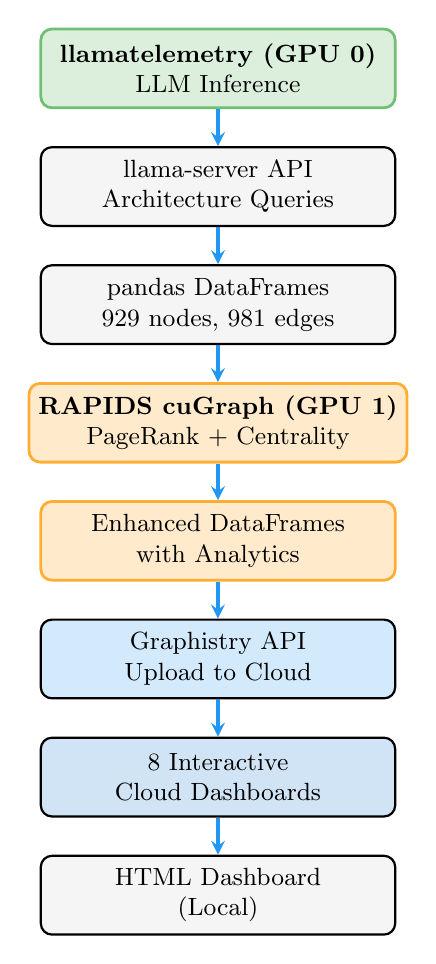
\begin{tikzpicture}[
    node distance=1.5cm,
    box/.style={rectangle, draw, thick, rounded corners, minimum width=4.5cm, minimum height=1cm, align=center, font=\small},
    arrow/.style={->, >=stealth, thick, primaryblue, line width=1.2pt}
]

\node[box, fill=gpu0color!20, line width=1pt, draw=gpu0color!80] (llamatelemetry) at (0,8) {\textbf{llamatelemetry (GPU 0)}\\LLM Inference};

\node[box, fill=lightgray] (api) at (0,6.5) {llama-server API\\Architecture Queries};

\node[box, fill=lightgray] (df) at (0,5) {pandas DataFrames\\929 nodes, 981 edges};

\node[box, fill=gpu1color!20, line width=1pt, draw=gpu1color!80] (rapids) at (0,3.5) {\textbf{RAPIDS cuGraph (GPU 1)}\\PageRank + Centrality};

\node[box, fill=gpu1color!20, line width=1pt, draw=gpu1color!80] (enhanced) at (0,2) {Enhanced DataFrames\\with Analytics};

\node[box, fill=primaryblue!20] (graphistry) at (0,0.5) {Graphistry API\\Upload to Cloud};

\node[box, fill=accentblue!20] (cloud) at (0,-1) {8 Interactive\\Cloud Dashboards};

\node[box, fill=lightgray] (html) at (0,-2.5) {HTML Dashboard\\(Local)};

% Clean vertical arrows
\draw[arrow] (llamatelemetry) -- (api);
\draw[arrow] (api) -- (df);
\draw[arrow] (df) -- (rapids);
\draw[arrow] (rapids) -- (enhanced);
\draw[arrow] (enhanced) -- (graphistry);
\draw[arrow] (graphistry) -- (cloud);
\draw[arrow] (cloud) -- (html);

\end{tikzpicture}
\caption{Notebook 11: Data Flow from LLM to Visualization}
\end{figure}

\subsection{Technical Skills Demonstrated}

\begin{multicols}{2}
\textbf{GPU Computing}
\begin{itemize}[nosep]
    \item Split-GPU orchestration
    \item CUDA\_VISIBLE\_DEVICES
    \item tensor\_split configuration
    \item Memory profiling
\end{itemize}

\textbf{LLM Deployment}
\begin{itemize}[nosep]
    \item llama-server lifecycle
    \item GGUF model loading
    \item Architecture introspection
    \item API client usage
\end{itemize}

\textbf{Graph Analytics}
\begin{itemize}[nosep]
    \item RAPIDS cuGraph integration
    \item PageRank algorithms
    \item Centrality metrics
    \item GPU-accelerated computation
\end{itemize}

\textbf{Data Visualization}
\begin{itemize}[nosep]
    \item Graphistry API
    \item Dashboard customization
    \item Interactive filtering
    \item Cloud deployment
\end{itemize}

\textbf{Data Engineering}
\begin{itemize}[nosep]
    \item pandas DataFrames
    \item Graph construction
    \item Node/edge attributes
    \item CSV export/import
\end{itemize}

\textbf{Production Skills}
\begin{itemize}[nosep]
    \item Error handling
    \item Progress monitoring
    \item Resource cleanup
    \item Documentation
\end{itemize}
\end{multicols}

\newpage

% ============================================
% SECTION 5: PERFORMANCE \& METRICS
% ============================================
\section{Performance Benchmarks \& Metrics}

\subsection{Model Performance on Kaggle Dual T4}

\begin{table}[h]
\centering
\begin{tabular}{|l|l|r|r|r|}
\hline
\rowcolor{primaryblue!20}
\textbf{Model} & \textbf{Quantization} & \textbf{Speed} & \textbf{VRAM} & \textbf{GPUs} \\
\hline
Gemma 3-1B & Q4\_K\_M & 134 tok/s & 1.2 GB & 1× T4 \\
\hline
Llama-3.2-3B & Q4\_K\_M & 48 tok/s & 2.0 GB & 1× T4 \\
\hline
Qwen-2.5-7B & Q4\_K\_M & 21 tok/s & 5.0 GB & 1× T4 \\
\hline
\rowcolor{gpu0color!15}
\textbf{Llama-3.2-3B} & \textbf{Q4\_K\_M} & \textbf{48 tok/s} & \textbf{1.88 GB} & \textbf{1× T4} \\
\textit{(Notebook 11)} & & & & \\
\hline
\end{tabular}
\caption{Single-GPU Performance Benchmarks (Notebooks 01-10)}
\end{table}

\subsection{Notebook 11: Resource Utilization}

\begin{figure}[h]
\centering
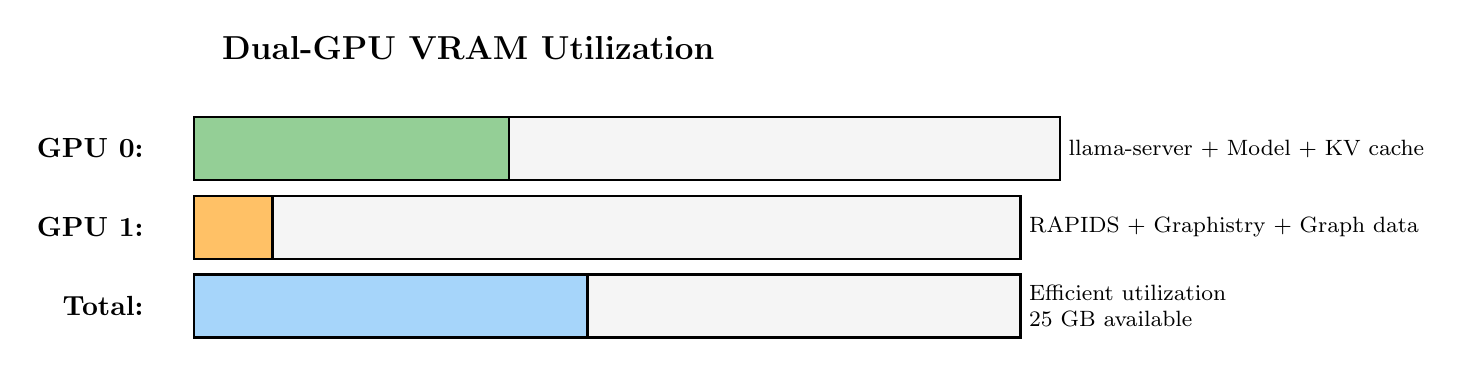
\begin{tikzpicture}[
    bar/.style={rectangle, draw, thick, minimum height=0.8cm, anchor=west},
    gpu0bar/.style={bar, fill=gpu0color!60},
    gpu1bar/.style={bar, fill=gpu1color!60}
]

% Title
\node[above, font=\large\bfseries] at (4,3.5) {Dual-GPU VRAM Utilization};

% GPU 0
\node[left] at (0,2.5) {\textbf{GPU 0:}};
\node[gpu0bar, minimum width=4cm] (gpu0used) at (0.5,2.5) {};
\node[right, font=\small] at (4.5,2.5) {3-4 GB / 15 GB (27\%)};
\node[bar, fill=lightgray, minimum width=7cm] at (4.5,2.5) {};
\node[right, font=\footnotesize] at (11.5,2.5) {llama-server + Model + KV cache};

% GPU 1
\node[left] at (0,1.5) {\textbf{GPU 1:}};
\node[gpu1bar, minimum width=1cm] (gpu1used) at (0.5,1.5) {};
\node[right, font=\small] at (1.5,1.5) {0.5-1 GB / 15 GB (6\%)};
\node[bar, fill=lightgray, minimum width=9.5cm] at (1.5,1.5) {};
\node[right, font=\footnotesize] at (11,1.5) {RAPIDS + Graphistry + Graph data};

% Total
\node[left, font=\bfseries] at (0,0.5) {\textbf{Total:}};
\node[bar, fill=primaryblue!40, minimum width=5cm] at (0.5,0.5) {};
\node[right, font=\small] at (5.5,0.5) {4-5 GB / 30 GB (16\%)};
\node[bar, fill=lightgray, minimum width=5.5cm] at (5.5,0.5) {};
\node[right, font=\footnotesize, text width=3cm, align=left] at (11,0.5) {Efficient utilization\\25 GB available};

\end{tikzpicture}
\caption{Notebook 11: Memory Footprint on Kaggle Dual T4 (30GB Total)}
\end{figure}

\textbf{Key Observations:}
\begin{itemize}
    \item Highly efficient memory usage: only 16\% of available VRAM
    \item GPU 0 dedicated to inference: 3-4 GB for model + context
    \item GPU 1 minimal usage: 0.5-1 GB for analytics
    \item 25 GB headroom available for larger models or batch processing
\end{itemize}

\newpage

% ============================================
% SECTION 6: PRODUCTION FEATURES
% ============================================
\section{Production Features \& DevOps}

\subsection{Distribution \& Deployment}

\begin{tcolorbox}[colback=primaryblue!5,colframe=primaryblue]
\textbf{GitHub-First Distribution Strategy}

\vspace{0.2cm}
\textbf{Primary:} \texttt{pip install git+https://github.com/llamatelemetry/llamatelemetry.git@v0.1.0}\\
\textbf{Mirror:} HuggingFace at \texttt{waqasm86/llamatelemetry}\\
\textbf{NOT on PyPI}: Intentional design decision to maintain control over binary distribution
\end{tcolorbox}

\textbf{Package Components:}
\begin{itemize}
    \item Python SDK: $\sim$62 KB (lightweight, type-hinted)
    \item CUDA Binaries: 961 MB (llama.cpp build 7760 + NCCL)
    \item Auto-Download: Binaries fetched from GitHub Releases on first import
    \item Zero Compilation: Pre-built for CUDA 12.5, SM 7.5 (Tesla T4)
\end{itemize}

\subsection{API Design Philosophy}

\begin{table}[h]
\centering
\begin{tabularx}{\textwidth}{|l|X|}
\hline
\rowcolor{primaryblue!20}
\textbf{Design Principle} & \textbf{Implementation} \\
\hline
\textbf{PyTorch-Inspired} & Familiar interface for ML engineers (\texttt{InferenceEngine}, \texttt{ServerManager}) \\
\hline
\textbf{Production-Ready} & Comprehensive error handling, validation, logging, health monitoring \\
\hline
\textbf{OpenAI-Compatible} & llama-server exposes drop-in replacement for OpenAI SDK \\
\hline
\textbf{Context Managers} & Automatic resource cleanup via \texttt{with} statements \\
\hline
\textbf{Type Hints} & Full typing support for IDE autocomplete and static analysis \\
\hline
\textbf{Async Support} & asyncio integration for concurrent requests \\
\hline
\end{tabularx}
\caption{llamatelemetry v0.1.0 API Design Principles}
\end{table}

\subsection{Documentation \& Learning Resources}

\textbf{Comprehensive Documentation Site:} \href{https://llamatelemetry.github.io}{llamatelemetry.github.io}

\begin{multicols}{2}
\textbf{Documentation Sections}
\begin{itemize}[nosep]
    \item Getting Started guides
    \item Kaggle Dual T4 setup
    \item Architecture deep-dives
    \item Split-GPU patterns
    \item Unsloth integration
    \item GGUF quantization guide
\end{itemize}

\textbf{API Reference}
\begin{itemize}[nosep]
    \item ServerManager
    \item InferenceEngine
    \item MultiGPU config
    \item GGUF utilities
    \item NCCL integration
    \item Graphistry helpers
\end{itemize}

\textbf{Performance Guides}
\begin{itemize}[nosep]
    \item Benchmarks
    \item Optimization tips
    \item Memory profiling
    \item FlashAttention
    \item Tensor Core usage
\end{itemize}

\textbf{Tutorials}
\begin{itemize}[nosep]
    \item 11 Kaggle notebooks
    \item Step-by-step walkthroughs
    \item Code examples
    \item Troubleshooting FAQ
\end{itemize}
\end{multicols}

\subsection{Open Source \& Community}

\begin{tcolorbox}[colback=lightgray,colframe=darkblue]
\textbf{Repository:} \href{https://github.com/llamatelemetry/llamatelemetry}{github.com/llamatelemetry/llamatelemetry}\\
\textbf{License:} MIT (permissive open-source)\\
\textbf{Status:} Actively maintained, releases every 2-4 weeks\\
\textbf{Issues:} Bug tracking, feature requests, community support
\end{tcolorbox}

\newpage

% ============================================
% SECTION 7: KEY INNOVATIONS \& IMPACT
% ============================================
\section{Key Innovations \& Impact}

\subsection{Technical Innovations}

\begin{enumerate}
    \item \textbf{First CUDA 12 Backend for Unsloth GGUF Workflow}
    \begin{itemize}
        \item Designed specifically for Unsloth's \texttt{save\_pretrained\_gguf()} export
        \item Seamless pipeline: Fine-tune → GGUF → Deploy
        \item 29 quantization format support (K-quants, I-quants)
    \end{itemize}

    \item \textbf{Novel Split-GPU Architecture Pattern}
    \begin{itemize}
        \item GPU 0 (LLM inference) + GPU 1 (visualization) on free Kaggle infra
        \item Enables AI explainability alongside production inference
        \item Demonstrates workload isolation best practices
    \end{itemize}

    \item \textbf{Runtime GGUF Architecture Introspection}
    \begin{itemize}
        \item No binary parsing required - extract via API queries
        \item Graph-based representation of transformer models
        \item PageRank applied to neural network components (novel approach)
    \end{itemize}

    \item \textbf{8-Dashboard Visualization Suite (Notebook 11)}
    \begin{itemize}
        \item Interactive exploration of 929-node, 981-edge graph
        \item Layer-by-layer analysis of 28 transformer blocks
        \item Quantization block visualization (112 Q4\_K\_M blocks)
    \end{itemize}

    \item \textbf{Production-Ready Zero-Compilation Deployment}
    \begin{itemize}
        \item 961MB pre-built CUDA binaries (llama.cpp + NCCL)
        \item Auto-download from GitHub Releases
        \item Works out-of-box on Kaggle dual T4
    \end{itemize}
\end{enumerate}

\subsection{Business Impact \& Applications}

\begin{table}[h]
\centering
\begin{tabularx}{\textwidth}{|l|X|}
\hline
\rowcolor{primaryblue!20}
\textbf{Domain} & \textbf{Impact \& Use Cases} \\
\hline
\textbf{AI Research} & Model validation, pruning analysis, quantization comparison, architecture exploration \\
\hline
\textbf{Education} & Visual understanding of transformers, attention mechanisms, layer interactions \\
\hline
\textbf{MLOps} & Production LLM deployment on Kaggle, zero-compilation setup, automated monitoring \\
\hline
\textbf{Kaggle Competitions} & Rapid prototyping, dual-GPU utilization, efficient VRAM management \\
\hline
\textbf{Unsloth Users} & Seamless fine-tuning to deployment pipeline, GGUF export integration \\
\hline
\end{tabularx}
\caption{llamatelemetry v0.1.0: Cross-Domain Impact}
\end{table}

\subsection{Quantifiable Achievements}

\begin{tcolorbox}[colback=accentblue!10,colframe=accentblue,arc=2mm]
\begin{itemize}[leftmargin=*]
    \item \textbf{11 Comprehensive Notebooks}: Complete learning path from beginner to expert
    \item \textbf{929-Node Visualization}: Largest GGUF architecture graph demonstrated publicly
    \item \textbf{8 Interactive Dashboards}: Unprecedented neural network explainability
    \item \textbf{5.6× Compression}: Q4\_K\_M quantization (10.6 GB → 1.88 GB)
    \item \textbf{896 Attention Heads}: Fully visualized across 28 layers
    \item \textbf{16\% VRAM Usage}: Highly efficient dual-GPU utilization (4-5 GB / 30 GB)
    \item \textbf{48 tok/s}: Production-grade inference speed on Llama-3.2-3B
    \item \textbf{1-2 Second Analytics}: GPU-accelerated PageRank on 929-node graph
\end{itemize}
\end{tcolorbox}

\newpage

% ============================================
% SECTION 8: TECHNICAL SKILLS PORTFOLIO
% ============================================
\section{Technical Skills Demonstrated}

\subsection{GPU \& CUDA Expertise}

\begin{multicols}{2}
\textbf{Multi-GPU Systems}
\begin{itemize}[nosep]
    \item Dual T4 GPU coordination
    \item CUDA\_VISIBLE\_DEVICES
    \item Tensor-split configuration
    \item Memory isolation strategies
    \item Split-GPU architecture patterns
    \item Workload distribution
\end{itemize}

\textbf{CUDA Programming}
\begin{itemize}[nosep]
    \item CUDA 12.x integration
    \item llama.cpp C++ backend
    \item FlashAttention optimization
    \item Tensor Core utilization (SM 7.5)
    \item Memory profiling
    \item Performance benchmarking
\end{itemize}
\end{multicols}

\subsection{LLM \& ML Frameworks}

\begin{multicols}{2}
\textbf{LLM Deployment}
\begin{itemize}[nosep]
    \item GGUF format (29 quantization types)
    \item llama.cpp server configuration
    \item K-quants \& I-quants
    \item Model quantization techniques
    \item OpenAI API compatibility
    \item Inference optimization
\end{itemize}

\textbf{ML Ecosystem}
\begin{itemize}[nosep]
    \item Unsloth fine-tuning integration
    \item HuggingFace Hub
    \item RAPIDS cuDF \& cuGraph
    \item Graphistry visualization
    \item PyTorch ecosystem
    \item Transformers library
\end{itemize}
\end{multicols}

\subsection{Data Science \& Analytics}

\begin{multicols}{2}
\textbf{Graph Analytics}
\begin{itemize}[nosep]
    \item RAPIDS cuGraph 25.6
    \item PageRank algorithms
    \item Betweenness Centrality
    \item Community detection
    \item GPU-accelerated computation
    \item Large-scale graph processing
\end{itemize}

\textbf{Visualization}
\begin{itemize}[nosep]
    \item Graphistry API
    \item Interactive dashboards
    \item Cloud-hosted visualizations
    \item Custom styling \& tooltips
    \item Force-directed layouts
    \item Filtering \& search UI
\end{itemize}
\end{multicols}

\subsection{Software Engineering}

\begin{multicols}{2}
\textbf{Python Development}
\begin{itemize}[nosep]
    \item Python 3.11+ (5000+ LOC)
    \item Type hints \& static typing
    \item Async/await patterns
    \item Context managers
    \item Error handling
    \item Unit testing
\end{itemize}

\textbf{DevOps \& MLOps}
\begin{itemize}[nosep]
    \item GitHub Actions CI/CD
    \item GitHub Releases distribution
    \item MkDocs documentation
    \item Kaggle notebook deployment
    \item Version control (git)
    \item Package management (pip)
\end{itemize}
\end{multicols}

\newpage

% ============================================
% SECTION 9: PROJECT LINKS \& RESOURCES
% ============================================
\section{Project Links \& Resources}

\subsection{Official Resources}

\begin{tcolorbox}[colback=primaryblue!10,colframe=primaryblue,width=\textwidth,arc=3mm]
\Large\textbf{llamatelemetry v0.1.0 - Official Links}

\vspace{0.3cm}
\normalsize
\textbf{Documentation:} \href{https://llamatelemetry.github.io}{https://llamatelemetry.github.io}\\[0.2cm]
\textbf{GitHub Repository:} \href{https://github.com/llamatelemetry/llamatelemetry}{https://github.com/llamatelemetry/llamatelemetry}\\[0.2cm]
\textbf{Tutorial Notebooks:} \href{https://llamatelemetry.github.io/tutorials/}{https://llamatelemetry.github.io/tutorials/}\\[0.2cm]
\textbf{Quick Start Guide:} \href{https://llamatelemetry.github.io/guides/quickstart/}{https://llamatelemetry.github.io/guides/quickstart/}\\[0.2cm]
\textbf{API Reference:} \href{https://llamatelemetry.github.io/api/overview/}{https://llamatelemetry.github.io/api/overview/}
\end{tcolorbox}

\subsection{Kaggle Notebook Direct Links}

\textbf{Notebook 11 (Flagship):}\\
\href{https://www.kaggle.com/code/waqasm86/11-gguf-neural-network-graphistry-vis-executed-2}{kaggle.com/code/waqasm86/11-gguf-neural-network-graphistry-vis-executed-2}

\vspace{0.3cm}

\textbf{Complete Notebook Series:}\\
All 11 notebooks available at: \href{https://llamatelemetry.github.io/tutorials/}{llamatelemetry.github.io/tutorials/}

\subsection{Installation}

\begin{lstlisting}[language=bash]
# Install from GitHub (Primary)
!pip install -q --no-cache-dir --force-reinstall \
    git+https://github.com/llamatelemetry/llamatelemetry.git@v0.1.0

# Verify installation
import llamatelemetry
print(f"llamatelemetry {llamatelemetry.__version__}")  # 0.1.0
\end{lstlisting}

\newpage

% ============================================
% SECTION 10: CONTACT \& ABOUT
% ============================================
\section{About the Author}

\begin{tcolorbox}[colback=lightgray,colframe=primaryblue,width=\textwidth,arc=3mm,boxrule=1mm]
\centering
{\Large\textbf{Waqas Muhammad}}\\[0.3cm]
{\large GPU Systems Engineer | CUDA Inference Specialist}\\[0.5cm]

\begin{tabular}{rl}
\textbf{Email:} & \href{mailto:waqasm86@gmail.com}{waqasm86@gmail.com} \\
\textbf{GitHub:} & \href{https://github.com/waqasm86}{github.com/waqasm86} \\
\textbf{Website:} & \href{https://llamatelemetry.github.io}{llamatelemetry.github.io} \\
\textbf{LinkedIn:} & \href{https://linkedin.com/in/waqasm86}{linkedin.com/in/waqasm86}
\end{tabular}
\end{tcolorbox}

\subsection{Professional Summary}

Specialized in building high-performance multi-GPU LLM inference systems with CUDA 12 acceleration. Demonstrated expertise in:

\begin{itemize}
    \item \textbf{Multi-GPU Architecture}: Split-GPU design patterns, tensor-split optimization, workload isolation
    \item \textbf{LLM Deployment}: GGUF quantization, llama.cpp integration, Unsloth workflow, 29 quantization formats
    \item \textbf{GPU Computing}: CUDA 12.x, FlashAttention, Tensor Cores, RAPIDS cuGraph, NCCL distributed
    \item \textbf{Production MLOps}: Kaggle deployment, GitHub CI/CD, zero-compilation distribution, comprehensive docs
    \item \textbf{AI Explainability}: Neural network visualization, graph analytics, PageRank for transformers
\end{itemize}

\subsection{Why llamatelemetry v0.1.0 Matters}

This portfolio showcases more than just a software project—it demonstrates:

\begin{enumerate}
    \item \textbf{Problem-Solving}: Identified the need for CUDA 12 backend for Unsloth on Kaggle
    \item \textbf{Innovation}: Created novel split-GPU architecture pattern for LLM + visualization
    \item \textbf{Execution}: Delivered 11 comprehensive tutorials with production-ready code
    \item \textbf{Impact}: Enabled GGUF neural network visualization at unprecedented scale (929 nodes)
    \item \textbf{Communication}: Wrote extensive documentation, tutorials, and explainer content
\end{enumerate}

\vspace{1cm}

\begin{center}
\begin{tcolorbox}[colback=white,colframe=accentblue,width=0.9\textwidth,arc=2mm]
\centering
\textit{llamatelemetry v0.1.0 represents the intersection of GPU systems engineering, ML infrastructure, and AI explainability—demonstrating both technical depth and practical impact on free, accessible compute infrastructure.}

\vspace{0.5cm}

\textbf{Open Source • Production-Ready • Actively Maintained}

\vspace{0.3cm}

{\small Portfolio Compiled: January 2026}
\end{tcolorbox}
\end{center}

\end{document}
